\ifx\wholebook\relax \else
\documentclass[b5paper]{article}
\usepackage[nomarginpar
  %, margin=.5in
]{geometry}

\addtolength{\oddsidemargin}{-0.05in}
\addtolength{\evensidemargin}{-0.05in}
\addtolength{\textwidth}{0.1in}
\usepackage[en]{../../../prelude}

\setcounter{page}{1}

\begin{document}

\title{Sequence}

\author{Xinyu~LIU
\thanks{{\bfseries Xinyu LIU} \newline
  Email: liuxinyu95@gmail.com \newline}
  }

\maketitle
\fi

\markboth{Sequence}{Elementary Algorithms}

\ifx\wholebook\relax
\chapter{Sequence}
\numberwithin{Exercise}{chapter}
\fi

\section{Introduction}
\label{introduction}

Sequence is a combination of array and list. We set the following goals for the ideal sequence:

\begin{enumerate}
\item Add, remove element on head and tail in constant time;
\item Fast (no slower than linear time) concatenate two sequences;
\item Fast access, update element at any position;
\item Fast split at any position;
\end{enumerate}

Array and list only satisfy these goals partially as shown in below table. Where $n$ is the length for the sequence. If there are two sequences, then we use $n_1$, $n_2$ for their lengths respectively.

\btab{| l | c | r |}
  \hline
  operation & array & list \\
  \hline
  add/remove on head & $O(n)$ & $O(1)$ \\
  add/remove on tail & $O(1)$ & $O(n)$ \\
  concatenate & $O(n_2)$ & $O(n_1)$ \\
  random access at $i$ & $O(1)$ & $O(i)$ \\
  remove at $i$ & $O(n-i)$ & $O(i)$ \\
  \hline
\etab

We give three implementations: binary random access list, concatenate-able list, and finger tree.

\section{Binary random access list}
\index{Sequence!Binary random access list}

The binary random access list is a set of full binary trees (forest). The elements are stored in leaves. For any integer $n \geq 0$, we know how many trees need to hold $n$ elements from its binary format. Every bit of 1 represents a binary tree, the tree size is determined by the magnitude of the bit. For any index $1 \leq i \leq n$, we can locate the binary tree that stores the $i$-th element. As shown in figure \ref{fig:bi-tree-sequence}, tree $t_1, t_2$ represent sequence $[x_1, x_2, x_3, x_4, x_5, x_6]$.

\begin{figure}[htbp]
  \centering
  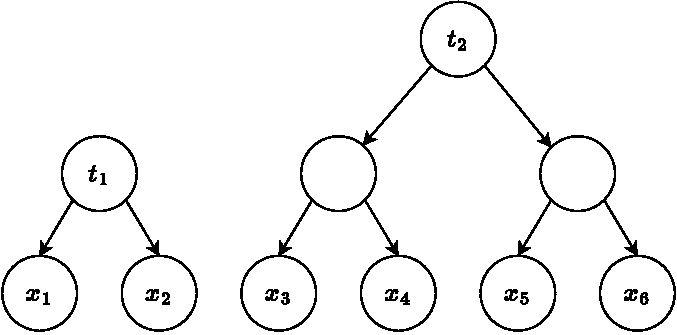
\includegraphics[scale=0.5]{img/bi-tree-sequence}
  \caption{A sequence of 6 elements.}
  \label{fig:bi-tree-sequence}
\end{figure}

Denote the full binary tree of depth $i + 1$ as $t_i$. $t_0$ only has a leaf node. There are $2^i$ leaves in $t_i$. For sequence of $n$ elements, represent $n$ in binary as $n = (e_m e_{m-1} ... e_1 e_0)_2$, where $e_i$ is either 1 or 0.

\be
n = 2^0 e_0 + 2^1 e_1 + ... + 2^m e_m
\ee

If $e_i \neq 0$, there is a full binary tree $t_i$ of size $2^i$. For example in figure \ref{fig:bi-tree-sequence}, the length of the sequence is $6 = (110)_2$. The lowest bit is 0, there's no tree of size 1; the 2nd bit is 1, there is $t_1$ of size 2; the highest bit is 1, there is $t_2$ of size 4. In this way, we represent sequence $[x_1, x_2, ..., x_n]$ as a list of trees. Each tree has unique size, in ascending order. We call it {\em binary random access list}\cite{okasaki-book}. We can customize the binary tree definition: (1) only store the element in leaf node as $(x)$; (2) augment the size in each branch node as $(s, l, r)$, where $s$ is the size of the tree, $l$, $r$ are left and right tree respectively. We get the size information as below:

\be
\begin{array}{rcl}
size\ (x) & = & 1 \\
size\ (s, l, r) & = & s \\
\end{array}
\ee

\index{Binary Random Access List!insert}
To add a new element $y$ before sequence $S$, we create a singleton $t_0$ tree $t' = (y)$, then insert it to the forest. $insert\ y\ S = insert_T\ (y)\ S$, or define it in Curried form:

\be
insert\ y = insert_T\ (y)
\ee

We compare $t'$ with the first tree $t_i$ in the forest, if $t_i$ is bigger, then put $t'$ ahead of the forest (in constant time); if they have the same size, then link them to a bigger tree (in constant time): $t'_{i+1} = (2s, t_i, t')$, then recursively insert $t'_{i+1}$ to the forest, as shown in figure \ref{fig:bralist-2}.

\be
\begin{array}{rcl}
insert_T\ t\ [\ ] & = & [t] \\
insert_T\ t\ (t_1 \cons ts) & = & \begin{cases}
  size\ t < size\ t_1: & t : t_1 : ts \\
  \text{otherwise}: & insert_T\ (link\ t\ t_1)\ ts \\
  \end{cases}
\end{array}
\ee

Where $link$ links two trees of the same size: $link\ t_1\ t_2 = (size\ t_1 + size\ t_2, t_1, t_2)$.

\begin{figure}[htbp]
  \centering
  \subcaptionbox{Insert $x_1$}{\hspace{0.2\textwidth}\includegraphics[scale=0.5]{img/bralst-1}\hspace{0.2\textwidth}}
  \subcaptionbox{Insert $x_2$, link to $[t_1]$.}{\hspace{0.2\textwidth}\includegraphics[scale=0.5]{img/bralst-2}\hspace{0.2\textwidth}} \\
  \subcaptionbox{Insert $x_3$, result $[t_0, t_1]$.}{\hspace{0.2\textwidth}\includegraphics[scale=0.5]{img/bralst-3}\hspace{0.2\textwidth}}
  \subcaptionbox{Insert $x_4$, link twice, generate $[t_2]$.}{\includegraphics[scale=0.5]{img/bralst-4}}
  \subcaptionbox{Insert $x_5$, result $[t_0, t_2]$.}{\includegraphics[scale=0.5]{img/bralst-5}}
  \subcaptionbox{Insert $x_6$, result $[t_1, t_2]$.}{\includegraphics[scale=0.5]{img/bralst-6}} \\
  \caption{Insert $x_1, x_2, ..., x_6$.}
  \label{fig:bralist-2}
\end{figure}

For $n$ elements, there are $m = O(\lg n)$ trees in the forest. The performance is bound to $O(\lg n)$ time. We'll prove the amortized performance is constant time.

\index{Binary Random Access List!remove}

Symmetrically, we can reverse the insert process to define remove. If the first tree is $t_0$ (singleton leaf), we remove $t_0$; otherwise, we repeat splitting the first tree to obtain a $t_0$ and remove it, as shown in figure \ref{fig:bralist-pop}.

\begin{figure}[htbp]
  \centering
  \subcaptionbox{Sequence $x_1, x_2, ..., x_5$ as $[t_0, t_2]$.}{\includegraphics[scale=0.5]{img/bralst-5}}
  \subcaptionbox{Remove $x_5$. Remove $t_0$ directly.}{\includegraphics[scale=0.5]{img/bralst-4}} \\
  \subcaptionbox{Remove $x_4$. Split twice to get $[t_0, t_0, t_1]$, then remove the head to get $[t_0, t_1]$.}{\hspace{0.2\textwidth}\includegraphics[scale=0.5]{img/bralst-3}\hspace{0.2\textwidth}}
  \caption{Remove}
  \label{fig:bralist-pop}
\end{figure}

\be
\begin{array}{rcl}
extract\ ((x) \cons ts) & = & (x, ts) \\
extract\ ((s, t_1, t_2) \cons ts) & = & extract\ (t_1 \cons t_2 \cons ts) \\
\end{array}
\ee

We call $extract$ to remove element from head:

\be
\begin{cases}
head & = \textit{fst} \circ extract \\
tail & = \textit{snd} \circ extract \\
\end{cases}
\ee

Where $\textit{fst}\ (a, b) = a$, $\textit{snd}\ (a, b) = b$ access the component in a pair.

\index{Binary Random Access List!random access}

The trees divides elements into chunks. For a given index $1 \leq i \leq n$, we first locate the corresponding tree, then lookup the tree to access the element.

\begin{enumerate}
\item For the first tree $t$ in the forest, if $i \leq size(t)$, then the element is in $t$, we next lookup $t$ for the target element;
\item Otherwise, let $i' = i - size(t)$, then recursively lookup the $i'$-th element in the rest trees.
\end{enumerate}

\be
(t \cons ts)[i] = \begin{cases}
  i \leq size\ t: & lookup_T\ i\ t \\
  \text{otherwise}: & ts[i - size\ t] \\
\end{cases}
\ee

Where $lookup_T$ applies binary search. If $i = 1$, returns the root, else divides the tree and recursively lookup:

\be
\begin{array}{rcl}
lookup_T\ 1\ (x) & = & x \\
lookup_T\ i\ (s, t_1, t_2) & = & \begin{cases}
  i \leq \lfloor \dfrac{s}{2} \rfloor: & lookup_T\ i\ t_1 \\
  \text{otherwise}: & lookup_T\ (i - \lfloor \dfrac{s}{2} \rfloor)\ t_2 \\
  \end{cases}
\end{array}
\ee

Figure \ref{fig:get-at-example} gives the steps to lookup the 4-th element in a sequence of length 6. The size of the first tree is 2 < 4, move to the next tree and update the index to $i' = 4 - 2$. The size of the second tree is $4 > i' = 2$, we need lookup it. Because the index 2 is less than the half size $4/2 = 2$, we lookup the left, then the right, and finally locate the element. Similarly, we can alter an element at a given position.

\begin{figure}[htbp]
  \centering
  \subcaptionbox{$S[4], 4 > size(t_1) = 2$}{\includegraphics[scale=0.5]{img/bralst-6}}
  \subcaptionbox{$S'[4-2] \Rightarrow lookup_T\ 2\ t_2$}{\hspace{0.2\textwidth}\includegraphics[scale=0.5]{img/bralst-4}\hspace{0.2\textwidth}} \\
  \subcaptionbox{$ 2 \leq \lfloor \dfrac{size(t_2)}{2} \rfloor \Rightarrow lookup_T\ 2\ left(t_2)$}{\hspace{0.2\textwidth}\includegraphics[scale=0.5]{img/bralst-4l}\hspace{0.2\textwidth}}
  \subcaptionbox{$lookup_T\ 1\ right(left(t_2))$, return $x_3$}{\hspace{0.2\textwidth}\includegraphics[scale=0.5]{img/bralst-4lr}\hspace{0.2\textwidth}}
  \caption{Steps to access $S[4]$}
  \label{fig:get-at-example}
\end{figure}

There are $O(\lg n)$ full binary trees to hold $n$ elements. For index $i$, we need at most $O(\lg n)$ time to locate the tree, the next lookup time is proportion to the height, which is $O(\lg n)$ at most. The overall random access time is bound to $O(\lg n)$.

\begin{Exercise}
How to handle the out of bound exception?
\end{Exercise}

\section{Numeric representation}
\index{Sequence!numeric representation}

The binary form of $n = 2^0e_0 + 2^1e_1 + ... + 2^me_m$ maps to the forest. The $e_i$ is the $i$-th bit. If $e_i = 1$, there is a full binary tree of size $2^i$. Adding an element corresponds to +1 to a binary number; while deleting corresponds to -1. We call such correspondence {\em numeric representation}\cite{okasaki-book}. To explicitly express this correspondence, we define two states: $Zero$ means none existence of the binary tree, while $One\ t$ means there exits tree $t$. As such, we represent the forest as a list of binary states, and implement insert as binary add.

\be
\begin{array}{rcl}
add\ t\ [\ ] & = & [One\ t] \\
add\ t\ (Zero \cons ds) & = & (One\ t) : ds \\
add\ t\ (One\ t' \cons ds) & = & Zero : add\ (link\ t\ t')\ ds
\end{array}
\ee

When add tree $t$, if the forest is empty, we create a state of $One\ t$, it's the only bit, corresponding to $0 + 1 = 1$. If the forest isn't empty, and the first bit is $Zero$, we use the state $One\ t$ to replace $Zero$, corresponding to binary add $(...digits...0)_2 + 1 = (...digits...1)_2$. For e.g. $6 + 1 = (110)_2 + 1 = (111)_2 = 7$. If the first bit is $One\ t'$, we assume $t$ and $t'$ have the same size because we always start to insert from a singleton leaf $t_0 = (x)$. The tree size increase as a sequence of $1, 2, 4, ..., 2^i, ...$. We link $t$ and $t'$, recursively insert to the rest bits. The original $One\ t'$ is replaced by $Zero$. It corresponds to binary add $(...digits...1)_2 + 1 = (...digits'...0)_2$. For e.g. $7 + 1 = (111)_2 + 1 = (1000)_2 = 8$.

Symmetrically, we can implement remove as binary subtraction. If the sequence is a singleton bit $One\ t$, it becomes empty after remove, corresponding to $1 - 1 = 0$. If there are multiple bits and the first one is $One\ t$, we replace it by $Zero$. This corresponds to $(...digits...1)_2 - 1 = (...digits...0)_2$. For e.g., $7 - 1 = (111)_2 - 1 = (110)_2 = 6$. If the first bit is $Zero$, we need borrow. We cursively extract tree from the rest bits, split into two $t_1, t_2$, replace $Zero$ to $One\ t_2$, and remove $t_1$. It corresponds to $(...digits...0)_2 - 1 = (...digits'...1)_2$. For e.g., $4 - 1 = (100)_2 - 1 = (11)_2 = 3$.

\be
\begin{array}{rcl}
minus\ [One\ t] & = & (t, [\ ]) \\
minus\ ((One\ t) \cons ts) & = & (t, Zero \cons ts) \\
minus\ (Zero \cons ts) & = & (t_1, (One\ t_2) \cons ts'), \text{where}: (s, t_1, t_2) = minus\ ts \\
\end{array}
\ee

Numeric representation doesn't change the performance. We next evaluate the amortized time by aggregation. The steps to insert $n = 2^m$ elements to empty is given as table \ref{tab:ralist-insertion}:

\begin{table}[htbp]
\centering
\begin{tabular}{| l | r |}
  \hline
  i & binary (MSB ... LSB) \\
  \hline
  0 & 0, 0, ..., 0, 0 \\
  1 & 0, 0, ..., 0, 1 \\
  2 & 0, 0, ..., 1, 0 \\
  3 & 0, 0, ..., 1, 1 \\
  ... & ... \\
  $2^m-1$ & 1, 1, ..., 1, 1 \\
  $2^m$ & 1, 0, 0, ..., 0, 0 \\
  \hline
  bits changed & 1, 1, 2, ... $2^{m-1}$, $2^m$ \\
  \hline
\end{tabular}
\caption{Insert $2^m$ elements.}
\label{tab:ralist-insertion}
\end{table}

The LSB changes every time when insert, total $2^m$ times. The second bit changes every other time (link trees), total $2^{m - 1}$ times. The second highest bit only changes 1 time, links all trees to a final one. The highest bit changes to 1 after insert the last element. Sum all times: $T = 1 + 1 + 2 + 4 + ... + 2^{m-1} + 2^m = 2^{m+1}$. Hence the amortized performance is:

\be
O(T/n) = O(\dfrac{2^{m+1}}{2^m}) = O(1)
\ee

Proved the amortized constant time performance.

\begin{Exercise}
\Question{Implement the random access for numeric representation $S[i], 1 \leq i \leq n$, where $n$ is the length of the sequence.}
\Question{Prove the amortized performance of delete is constant time. (hint: use aggregation method).}
\Question{We can represent the full binary tree with array of length $2^m$, where $m$ is none negative integer. Implement the binary tree forest, insert, and random access. What are the performance?}
\end{Exercise}

\section{paired-array sequence}
\index{Sequence!Paired-array sequence}

We give paired-array queue in chapter 11. We can expand it to paired-array sequence as array supports random access. As shown in figure \ref{fig:parrays}, we link two arrays head to head. When add an element from left, we append to the tail of $f$; when add from right, we append to the tail of $r$. We denote the sequence as a pair $S = (f, r)$, $\textproc{Front}(S) = f$, $\textproc{Rear}(S) = r$ access them respectively. We implement insert/append as below:

\begin{figure}[htbp]
  \centering
  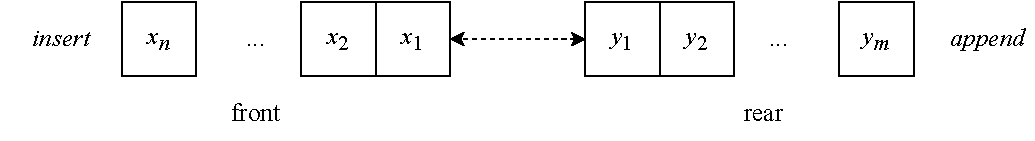
\includegraphics[scale=0.7]{img/parrays}
  \caption{Paired-array sequence.}
  \label{fig:parrays}
\end{figure}

\begin{algorithmic}[1]
\Function{Insert}{$x, S$}
  \State \textproc{Append}($x$, \Call{Front}{$S$})
\EndFunction
%\Statex
\Function{Append}{$x, S$}
  \State \textproc{Append}($x$, \Call{Rear}{$S$})
\EndFunction
\end{algorithmic}

\index{Paired-array sequence!random access}

When access the $i$-th element, we first determine $i$ index to $f$ or $r$, then locate the position. If $ i \leq |f|$, the element is in $f$. Because $f$ and $r$ are connected head to head, we need index from right of $f$ at position $|f| - i + 1$; if $i > |f|$, the element is in $r$. We index from left at position $i - |f|$.

\begin{algorithmic}[1]
\Function{Get}{$i, S$}
  \State $f, r \gets $ \Call{Front}{$S$}, \Call{Rear}{$S$}
  \State $n \gets $ \Call{Size}{$f$}
  \If{$i \leq n $}
    \State \Return $f[n - i + 1]$ \Comment{reversed}
  \Else
    \State \Return $r[i - n]$
  \EndIf
\EndFunction
\end{algorithmic}

\index{Paired-array sequence!remove and balance}
Removing can makes $f$ or $r$ empty ($[\ ]$), while the other is not. To re-balance, we halve the none empty one, and reverse either half to form a new pair. As $f$ and $r$ are symmetric, we can swap them, call \textproc{Balance}, then swap back.

\begin{algorithmic}[1]
\Function{Balance}{$S$}
  \State $f \gets$ \Call{Front}{$S$}, $r \gets$ \Call{Rear}{$S$}
  \State $n \gets$ \Call{Size}{$f$}, $m \gets$ \Call{Size}{$r$}
  \If{$F = [\ ]$}
    \State $k \gets \lfloor \dfrac{m}{2} \rfloor$
    \State \Return $(\textproc{Reverse}(r[1 ... k]), r[(k + 1) ... m])$
  \EndIf
  \If{$R = [\ ]$}
    \State $k \gets \lfloor \dfrac{n}{2} \rfloor$
    \State \Return $(f[(k + 1) ... n], \textproc{Reverse}(f[1 ... k]))$
  \EndIf
  \State \Return $(f, r)$
\EndFunction
\end{algorithmic}

Every time when delete, we check $f$, $r$ and balance them:

\begin{algorithmic}[1]
\Function{Remove-Head}{$S$}
  \State \Call{Balance}{$S$}
  \State $f, r \gets$ \Call{Front}{$S$}, \Call{Rear}{$S$}
  \If{$f = [\ ]$} \Comment{$S = ([], [x])$}
    \State $r \gets [\ ]$
  \Else
    \State \Call{Remove-Last}{$f$}
  \EndIf
\EndFunction
\Statex
\Function{Remove-Tail}{$S$}
  \State \Call{Balance}{$S$}
  \State $f, r \gets$ \Call{Front}{$S$}, \Call{Rear}{$S$}
  \If{$r = [\ ]$} \Comment{$S = ([x], [])$}
    \State $f \gets [\ ]$
  \Else
    \State \Call{Remove-Last}{$r$}
  \EndIf
\EndFunction
\end{algorithmic}

Due to reverse, the performance is $O(n)$ in the worst case, where $n$ is the number of elements, while it is amortized constant time.

\begin{Exercise}
\Question{For paired-array delete, prove the amortized performance is constant time.}
\end{Exercise}

\section{Concatenate-able list}
\index{Sequence!Concatenate-able list}

We achieve $O(\lg n)$ time insert, delete, random index with binary tree forest. However, it's not easy to concatenate two sequences. We can't merely merge trees, but need link trees with the same size. Figure \ref{fig:clist} shows an implementation of concatenate-able list. The first element $x_1$ is in root, the rest is organized with smaller sequences, each one is a sub-tree. These sub-trees are put in a real-time queue (see chapter 11). We denote the sequence as $(x_1, Q_x) = [x_1, x_2, ..., x_n]$. When concatenate with another sequence of $(y_1, Q_y) = [y_1, y_2, ..., y_m]$, we append it to $Q_x$. The real-time queue guarantees the en-queue in constant time, hence the concatenate performance is in constant time.

\begin{figure}[htbp]
  \centering
  \subcaptionbox{$(x_1, Q_x) = [x_1, x_2, ..., x_n]$}{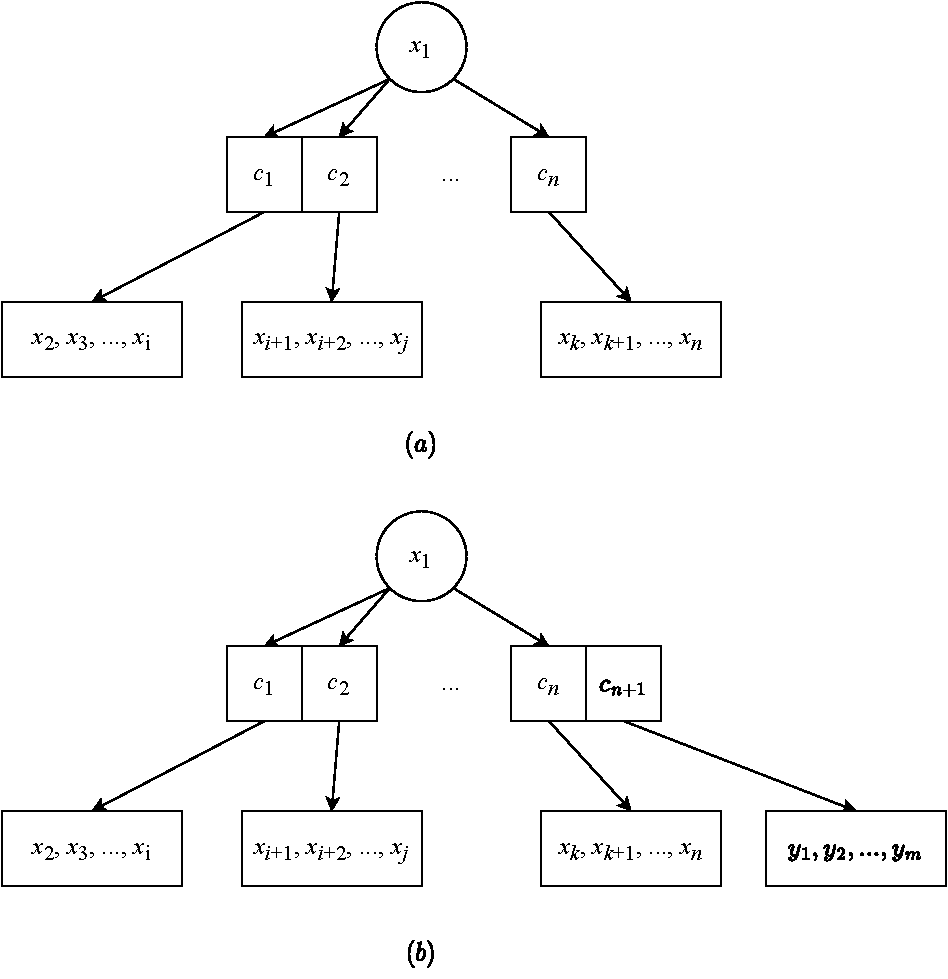
\includegraphics[scale=0.5]{img/clist}} \\
  \subcaptionbox{Concatenate with $(y_1, Q_y) = [y_1, y_2, ..., y_m]$, add$c_{n+1}$ to $Q_x$}{\includegraphics[scale=0.4]{img/clist1}}
  \caption{Concatenate-able list}
  \label{fig:clist}
\end{figure}

\be
\begin{array}{rcl}
s \doubleplus \nil & = & s \\
\nil \doubleplus s & = & s \\
(x, Q) \doubleplus s & = & (x,\ push\ s\ Q) \\
\end{array}
\ee

When insert new element $z$, we create a singleton of $(z, \nil)$, then concatenate it to the sequence:

\be
\begin{cases}
insert\ x\ s & = (x, \nil) \doubleplus s \\
append\ x\ s & = s \doubleplus (x, \nil) \\
\end{cases}
\ee

When delete $x_1$ from head, we lose the root. The rest sub-trees are all concatenate-able lists. We concatenate them all to a new sequence.

\be
\begin{array}{rcl}
concat\ \nil & = & \nil \\
concat\ Q & = & (top\ Q) \doubleplus concat\ (pop\ Q) \\
\end{array}
\ee

The real-time queue hold sub-trees, we pop the first $c_1$, and recursively concatenate the rest to $s$, then concatenate $c_1$ and $s$. We define delete from head with $concat$.

\be
tail\ (x, Q) = concat\ Q
\ee

Function $concat$ traverses the queue, and reduces to a result, it essentially folds on $Q$\cite{learn-haskell}.

\be
\begin{array}{rcl}
fold\ f\ z\ \nil & = & z \\
fold\ f\ z\ Q & = & f\ (top\ Q)\ (fold\ f\ z\ (pop\ Q)) \\
\end{array}
\ee

Where $f$ is a binary function, $z$ is zero unit. Here are examples of folding on queue $Q = [1, 2, ..., 5]$:

\[
\begin{array}{rcl}
fold\ (+)\ 0\ Q & = & 1 + (2 + (3 + (4 + (5 + 0)))) = 15 \\
fold\ (\times)\ 1\ Q\ & = & 1 \times (2 \times (3 \times (4 \times (5 \times 1)))) = 120 \\
fold\ (\times)\ 0\ Q & = & 1 \times (2 \times (3 \times (4 \times (5 \times 0)))) = 0 \\
\end{array}
\]

We can define $concat$ with fold (Curried form):

\be
concat = fold\ (\doubleplus)\ \nil
\ee

The performance is bound to linear time in worst case: delete after repeatedly add $n$ elements. All $n-1$ sub-trees are singleton. $concat$ takes $O(n)$ time to consolidate. The amortized performance is constant time if add, append, delete randomly happen.

\begin{Exercise}
\Question{Prove the amortized performance for delete is constant time} %Banker method.
\end{Exercise}

\section{Finger tree}
\index{Sequence!finger tree}

Binary random access list supports to insert, remove from head in amortized constant time, and index in logarithm time. But we can't easily append element to tail, or fast concatenate. With concatenate-able list, we can concatenate, insert, and append in amortized constant time, but can't easily index element. From these two examples, we need: 1, access head, tail fast to insert or delete; 2, the recursive structure, e.g., tree, realizes random access as divide and conquer search. Finger tree\cite{finger-tree-1977} implements sequence with these two ideas\cite{finger-tree-2006}. It's critical to maintain the tree balanced to guarantee search performance. Finger tree leverages 2-3 tree (a type of B-tree). A 2-3 tree is consist of 2 or 3 sub-trees, as $(t_1, t_2)$ or $(t_1, t_2, t_3)$.

\lstset{frame = single}
\begin{Haskell}
data Node a = Br2 a a | Br3 a a a
\end{Haskell}

We define a finger tree as one of below three:

\begin{enumerate}
\item empty $\nil$;
\item a singleton leaf $(x)$;
\item a tree with three parts: a sub-tree, left and right finger, denoted as $(f, t, r)$. Each finger is a list up to 3 elements\footnote{f: front, r: rear}.
\end{enumerate}

\begin{Haskell}
data Tree a = Empty
            | Lf a
            | Tr [a] (Tree (Node a)) [a]
\end{Haskell}

\subsection{Insert}

\begin{figure}[htbp]
  \centering
  \subcaptionbox{$\nil$}{\hspace{0.2\textwidth}\includegraphics[scale=0.5]{img/ftr-empty}\hspace{0.2\textwidth}}
  \subcaptionbox{$(x)$}{\hspace{0.2\textwidth}\includegraphics[scale=0.5]{img/ftr-leaf}\hspace{0.2\textwidth}} \\
  \subcaptionbox{$([b], \nil, [a])$}{\includegraphics[scale=0.5]{img/ftr-ab}}
  \caption{Finger tree, example 1}
  \label{fig:ftr-example-1}
\end{figure}

\begin{figure}[htbp]
  \centering
  \subcaptionbox{Insert 3 elements to $f$, not a valid, balanced 2-3 tree.}{\includegraphics[scale=0.5]{img/ftr-abcde}}
  \hspace{0.2\textwidth}
  \subcaptionbox{Re-balance. there are two elements in $f$; the middle is a singleton of a 2-3 tree.}{\includegraphics[scale=0.5]{img/ftr-abcdef}}
  \caption{Finger tree, example 2}
  \label{fig:ftr-example-2}
\end{figure}

As shown in figure \ref{fig:ftr-example-1} and \ref{fig:ftr-example-2}. Example 1 (a) is $\nil$, (b) is a singleton, (c) has two element in $f$ and $r$ for each. When add more, $f$ will exceeds 2-3 tree, as in example 2 (a). We need re-balance as in (b). There are two elements in $f$, the middle is singleton of a 2-3 tree. These examples are list as below:

\[
\begin{array}{ll}
\nil & \texttt{Empty}\\
(a) & \texttt{Lf a}\\
([b], \nil, [a]) & \texttt{Tr [b] Empty [a]}\\
([e, d, c, b], \nil, [a]) & \texttt{Tr [e, d, c, b] Empty [a]}\\
([f, e], (d, c, b), [a]) & \texttt{Tr [f, e] Lf (Br3 d c b) [a]}\\
\end{array}
\]

\index{Finger tree!insert to left}

In example 2 (b), the middle component is a singleton leaf. Finger tree is recursive, apart from $f$ and $r$, the middle is a deeper finger tree of type $Tree\ (Node\ a)$. One more wrap, one level deeper. Summarize above examples, we define insert $a$ to tree $T$ as below:

\begin{enumerate}
\item If $T = \nil$, the result is a singleton $(a)$;
\item If $T = (b)$ is a leaf, the result is $([a], \nil, [b])$;
\item For $T = (f, t, r)$, if there are $\leq 3$ elements in $f$, we insert $a$ to $f$, otherwise ($> 3$), extract the last 3 elements from $f$ to a 2-3 tree $t'$, recursively insert $t'$ to $t$, then insert $a$ to $f$.
\end{enumerate}

\be
\begin{array}{rcl}
insert\ a\ \nil & = & (x) \\
insert\ a\ (b) & = & ([a], \nil, [b]) \\
insert\ a\ ([b, c, d, e], t, r) & = & ([a, b], insert\ (c, d, e)\ t, r) \\
insert\ a\ (f, t, r) & = & (a \cons f, t, r) \\
\end{array}
\ee

The insert performance is constant time except for the recursive case. The recursion time is proportion to the height of the tree $h$. Because of 2-3 trees, it's balanced, hence $h = O(\lg n)$, where $n$ is the number of elements. When distribute the recursion to other cases, the amortized performance is constant time\cite{okasaki-book}\cite{finger-tree-2006}. We can repeatedly insert a list of elements by folding:

\be
xs \gg t = foldr\ insert\ t\ xs
\ee

\begin{Exercise}
\Question{Eliminate recursion, implement insert with loop.}
\end{Exercise}

\begin{Answer}
\Question{Eliminate recursion, implement insert with loop.

Let $\textproc{Mid}(T) = t$ access the middle part of tree $T = (f, t, r)$.

\begin{algorithmic}[1]
\Function{Insert}{$x, T$}
  \State $n = (x)$
  \State $\perp \gets p \gets ([\ ], T, [\ ])$
  \While{$|\textproc{Front}(T)| \geq 3$}
    \State $f \gets \textproc{Front}(T)$
    \State $n \gets (f[2], f[3], ...)$
    \State $\textproc{Front}(T) \gets [n, f[1]]$
    \State $p \gets T$
    \State $T \gets$ \Call{Mid}{$T$}
  \EndWhile
  \If{$T =$ NIL}
    \State $T \gets ([n], \text{NIL}, [\ ])$
  \ElsIf{ $|\textproc{Front}(T)| = 1$ and $\textproc{Rear}(T) = [\ ]$}
    \State \Call{Rear}{$T$} $\gets$ \Call{Front}{$T$}
    \State \Call{Front}{$T$} $\gets [n]$
  \Else
    \State \textproc{Insert}(\Call{Front}{$T$}, $n$)
  \EndIf
  \State \Call{Mid}{$p$} $\gets T$
  \State $T \gets$ \Call{Mid}{$\perp$}, \Call{Mid}{$\perp$} $\gets$ NIL
  \State \Return $T$
\EndFunction
\end{algorithmic}

We wrap $x$ in a leaf $(x)$. If there are more than 3 elements in $f$, we go top-down along the middle part. We extract the elements except the first one in $f$ out, wrap them in a node $n$ (depth + 1), then insert $n$ to the middle. We form $n$ and the remaining in $f$ as the new $f$ finger. At the end of traverse, we either reach an empty tree, or a tree can hold more elements in $f$. For empty tree case, we create a new leaf node; otherwise, we insert $n$ to the head of $f$. We return the root $T$. To simplify implementation, we create a special $\perp$ node as the parent of the root.}
\end{Answer}

\subsection{Extract}
\index{Finger tree!Remove from left}

We implement extract as the reverse of \textit{insert}.

\be
\begin{array}{rcl}
extract\ (a) & = & (a, \nil) \\
extract\ ([a], \nil, [b]) & = & (a, (b)) \\
extract\ ([a], \nil, b \cons bs) & = & (a, ([b], \nil, bs)) \\
extract\ ([a], t, r) & = & (a, (toList\ f, t', r)), \text{where}: (f, t') = extract\ t \\
extract\ (a \cons as, t, r) & = & (a, (as, t, r)) \\
\end{array}
\ee

Where \textit{toList} flatten a 2-3 tree to list:

\be
\begin{array}{rcl}
toList\ (a, b) & = & [a, b] \\
toList\ (a, b, c) & = & [a, b, c] \\
\end{array}
\ee

We skip error handling (e.g., extract from empty tree). If the tree is a singleton leaf, the result is empty; if there are two elements, the result is a singleton; if $f$ is a singleton list, the middle is empty, while $r$ isn't empty, we extract the only one in $f$, then borrow one from $r$ to $f$; if the middle isn't empty, we recursively extract a node from the middle, flatten that node to list to replace $f$ (the original one is extracted). If $f$ has more than one element, we extract the first. Figure \ref{fig:ftr-uncons-example} gives examples that extract 2 elements.


\begin{figure}[htbp]
  \centering
  \subcaptionbox{A sequence of 10 elements.}{\includegraphics[scale=0.4]{img/ftr-10}} \\
  \subcaptionbox{Extract one, $f$ becomes a singleton list.}{\includegraphics[scale=0.4]{img/ftr-9}} \\
  \subcaptionbox{Extract another, borrow an element from the middle, flatten the 2-3 tree to a list as the new $f$.}{\hspace{0.2\textwidth}\includegraphics[scale=0.4]{img/ftr-8}\hspace{0.2\textwidth}}
  \caption{Extract}
  \label{fig:ftr-uncons-example}
\end{figure}

We can define \textit{head}, \textit{tail} with \textit{extract}.

\be
\begin{cases}
head & = fst \circ extract \\
tail & = snd \circ extract \\
\end{cases}
\ee

\begin{Exercise}
\Question{Eliminate recursion, implement extract in loops.}
\end{Exercise}

\begin{Answer}
\Question{Eliminate recursion, implement extract in loops.

We borrow node from the middle when $f$ is empty. However, the tree may not well formed, e.g., both $f$ and the middle are empty. It is caused by splitting.

\begin{center}
  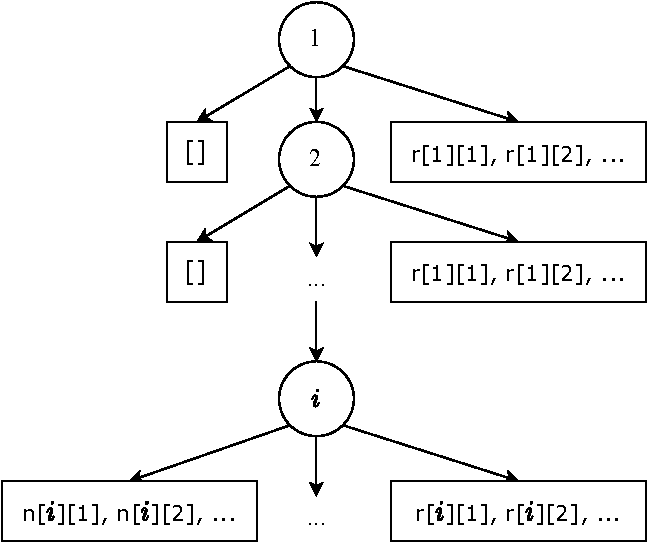
\includegraphics[scale=0.4]{img/ftr-illed-1}
  \captionof{figure}{The $f$ isn't empty at level $i$.}
  \label{fig:ftr-illed-form}
\end{center}

To extract the first element, we need a top-bottom pass, locate a sub-tree, either $f$ isn't empty, or both $f$ and the middle are empty as shown in figure \ref{fig:ftr-illed-form}. For the former, we extract the first node from $f$; for the latter, we swap $f$ and $r$, convert it to the former case. If the node extracted from $f$ isn't a leaf, we need go on extracting. We back track along the parent, till extract a leaf and reach to the root, as shown in figure \ref{fig:ftr-illed-extract}.

\begin{center}
  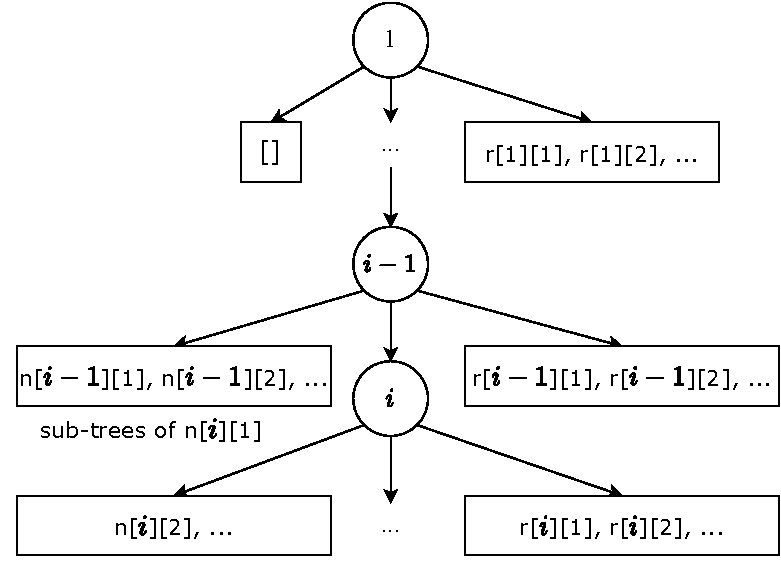
\includegraphics[scale=0.4]{img/ftr-illed-2} \\
  Extract the first $n[i][1]$, move its sub-tree to $f$ in upper level.\\
  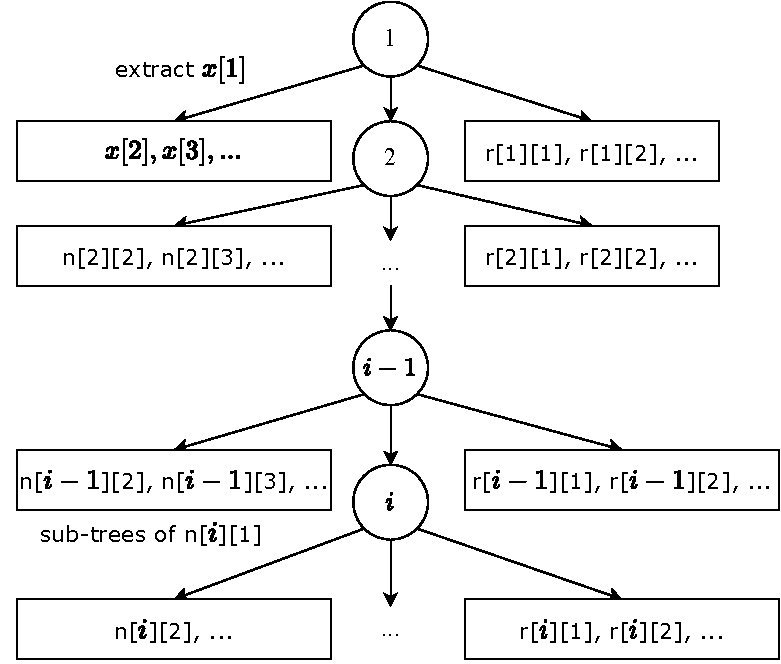
\includegraphics[scale=0.4]{img/ftr-illed-i} \\
  Repeat $i$ times, extract $x[1]$. \\
  \captionof{figure}{Bottom up back track to extract a leaf.}
  \label{fig:ftr-illed-extract}
\end{center}

Assume the tree isn't empty, we implement extract as below:

\begin{algorithmic}[1]
\Function{Extract}{$T$}
  \State $\perp \gets ([], T, [])$
  \While{\Call{Front}{$T$} $= [\ ]$ and \Call{Mid}{$T$} $\neq $ NIL}
    \State $T \gets$ \Call{Mid}{$T$}
  \EndWhile

  \If{\Call{Front}{$T$} $ = [\ ]$ and \Call{Rear}{$T$} $\neq [\ ]$}
    \State \textproc{Exchange} \Call{Front}{$T$} $\leftrightarrow$ \Call{Rear}{$T$}
  \EndIf

  \State $f \gets$ \Call{Front}{$T$}, $r \gets$ \Call{Rear}{$T$}
  \State $n \gets (f[1], f[2], ...)$ \Comment{$n$ is 2-3 tree}
  \Repeat
    \State \Call{Front}{$T$} $\gets [n_2, n_3, ..]$
    \State $n \gets n_1$
    \State $T \gets $ \Call{Parent}{$T$}
    \If{\Call{Mid}{$T$} becomes empty}
      \State \Call{Mid}{$T$} $\gets$ NIL
    \EndIf
  \Until{$n$ is leaf}
  \State \Return (\Call{Elem}{$n$}, \Call{Mid}{$\perp$})
\EndFunction
\end{algorithmic}

Where function \textproc{Elem}($n$) access the element in sub-tree $n$. We need change the way to access the first/last element of finger tree. If the finger is empty, and the middle isn't empty, we need search along the middle.

\begin{algorithmic}[1]
\Function{First-Leaf}{$T$}
  \While{\Call{Front}{$T$} $ = [\ ]$ and \Call{Mid}{$T$} $\neq$ NIL}
    \State $T \gets$ \Call{Mid}{$T$}
  \EndWhile
  \If{\Call{Front}{$T$} $ = [\ ]$ and \Call{Rear}{$T$} $\neq [\ ]$}
    \State $n \gets$ \Call{Rear}{$T$}[1]
  \Else
    \State $n \gets$ \Call{Front}{$T$}[1]
  \EndIf
  \While{$n$ is NOT leaf}
    \State $n \gets n_1$
  \EndWhile
  \State \Return $n$
\EndFunction
\Statex
\Function{First}{$T$}
  \State \Return \textproc{Elem}(\Call{First-Leaf}{$T$})
\EndFunction
\end{algorithmic}

In the second loop, if the node is not a leaf, we need traverse along the first sub-tree. The method to access the last element is symmetric.
}
\end{Answer}

\subsection{Append and remove}
\index{Finger tree!Append to tail}

Because finger tree is symmetric, we can give the realization of appending element on tail
by referencing to $insertT$ algorithm.

\be
appendT(T, x) = \left \{
  \begin{array}
  {r@{\quad:\quad}l}
  leaf(x) & T = \phi \\
  tree(\{y\}, \phi, \{x\}) & T = leaf(y) \\
  tree(F, appendT(M, tr3(x_1, x_2, x_3)), \{x_4, x\}) & T = tree(F, M, \{x_1, x_2, x_3, x_4\}) \\
  tree(F, M, R \cup \{x\}) & otherwise
  \end{array}
\right .
\ee

Generally speaking, if the rear finger is still valid 2-3 tree, that the number of elements
is not greater than 4, the new elements is directly appended to rear finger.
Otherwise, we break the rear finger, take the first 3 elements in rear finger to create a
new 2-3 tree, and recursively append it to the middle part inner tree.
If the finger tree is empty or a singleton leaf, it will be handled in the first two cases.

Translating the equation to Haskell yields the below program.

\lstset{language=Python}
\begin{lstlisting}
snoc :: Tree a -> a -> Tree a
snoc Empty a = Lf a
snoc (Lf a) b = Tr [a] Empty [b]
snoc (Tr f m [a, b, c, d]) e = Tr f (snoc m (Br3 a b c)) [d, e]
snoc (Tr f m r) a = Tr f m (r++[a])
\end{lstlisting}

Function name \texttt{snoc} is mirror of \texttt{cons}, which indicates the symmetric relationship.

Appending new element to the end imperatively is quite similar. The following algorithm
realizes appending.

\begin{algorithmic}
\Function{Append-Node}{$T, n$}
  \State $r \gets $ \textproc{Tree}()
  \State $p \gets r$
  \State \Call{Connect-Mid}{$p, T$}
  \While{\textproc{Full?}(\Call{Rear}{$T$})}
    \State $R \gets $ \Call{Rear}{$T$} \Comment{$R = \{n_1, n_2, ..., , n_{m-1}, n_m \}$}
    \State \Call{Rear}{$T$} $\gets$ $\{n, $ \Call{Last}{$R$} $\}$ \Comment{last element $n_m$}
    \State $n \gets$ \textproc{Node}()
    \State \Call{Children}{$n$} $\gets R[1...m-1]$ \Comment{ $\{n1, n2, ..., n_{m-1}\}$}
    \State $p \gets T$
    \State $T \gets$ \Call{Mid}{$T$}
  \EndWhile
  \If{$T =$ NIL}
    \State $T \gets$ \textproc{Tree}()
    \State \Call{Front}{$T$} $\gets \{ n \}$
  \ElsIf{ $|$ \Call{Rear}{$T$} $|$ = 1 $\land$ \Call{Front}{$T$} = $\phi$}
    \State \Call{Front}{$T$} $\gets$ \Call{Rear}{$T$}
    \State \Call{Rear}{$T$} $\gets \{ n \}$
  \Else
    \State \Call{Rear}{$T$} $\gets$ \Call{Rear}{$T$} $\cup \{ n \} $
  \EndIf
  \State \Call{Connect-Mid}{$p, T$} $\gets T$
  \State \Return \Call{Flat}{$r$}
\EndFunction
\end{algorithmic}

And the corresponding Python programs is given as below.

\lstset{language=Python}
\begin{lstlisting}
def append_node(t, n):
    root = prev = Tree()
    prev.set_mid(t)
    while rearFull(t):
        r = t.rear
        t.rear = r[-1:] + [n]
        n = wraps(r[:-1])
        prev = t
        t = t.mid
    if t is None:
        t = leaf(n)
    elif len(t.rear) == 1 and t.front == []:
        t = Tree(t.rear, None, [n])
    else:
        t = Tree(t.front, t.mid, t.rear + [n])
    prev.set_mid(t)
    return flat(root)
\end{lstlisting}

\subsection{remove element from the tail of the sequence}
\index{Finger tree!Remove from tail}

Similar to $appendT$, we can realize the algorithm which remove the last element from
finger tree in symmetric manner of $extractT$.

We denote the non-empty, non-leaf finger tree as $tree(F, M, R)$, where $F$ is the
front finger, $M$ is the middle part inner tree, and $R$ is the rear finger.

\be
removeT(T) = \left \{
  \begin{array}
  {r@{\quad:\quad}l}
  (\phi, x) & T = leaf(x) \\
  (leaf(y), x) & T = tree(\{y\}, \phi, \{x\}) \\
  (tree(init(F), \phi, last(F)), x) & T = tree(F, \phi, \{x\}) \land F \neq \phi \\
  (tree(F, M', toList(R')), x) & T = tree(F, M, \{x\}), (M', R') = removeT(M) \\
  (tree(F, M, init(R)), last(R)) & otherwise
  \end{array}
\right .
\ee

Function $toList(T)$ is used to flatten a 2-3 tree to plain list, which is defined
previously. Function $init(L)$ returns all elements except for the last one in list $L$,
that if $L = \{a_1, a_2, ..., a_{n-1}, a_n\}$, $init(L) = \{a_1, a_2, ..., a_{n-1}\}$.
And Function $last(L)$ returns the last element, so that $last(L) = a_n$. Please
refer to the appendix of this book for their implementation.

Algorithm $removeT()$ can be translated to the following Haskell program, we name
it as \texttt{unsnoc} to indicate it's the reverse function of \texttt{snoc}.

\lstset{language=Haskell}
\begin{lstlisting}
unsnoc :: Tree a -> (Tree a, a)
unsnoc (Lf a) = (Empty, a)
unsnoc (Tr [a] Empty [b]) = (Lf a, b)
unsnoc (Tr f@(_:_) Empty [a]) = (Tr (init f) Empty [last f], a)
unsnoc (Tr f m [a]) = (Tr f m' (nodeToList r), a) where (m', r) = unsnoc m
unsnoc (Tr f m r) = (Tr f m (init r), last r)
\end{lstlisting}

And we can define a special function \texttt{last} and \texttt{init} for finger tree which is similar
to their counterpart for list.

\begin{lstlisting}
last = snd . unsnoc
init = fst . unsnoc
\end{lstlisting}

Imperatively removing the element from the end is almost as same as removing on the head.
Although there seems to be a special case, that as we always store the only element (or sub node) in the front
finger while the rear finger and middle part inner tree are empty (e.g. $Tree(\{n\}, NIL, \phi)$),
it might get nothing if always try to fetch the last element from rear finger.

This can be solved by swapping the front and the rear finger if the rear is empty as in the
following algorithm.

\begin{algorithmic}
\Function{Extract-Tail}{$T$}
  \State $r \gets$ \textproc{Tree}()
  \State \Call{Connect-Mid}{$r, T$}
  \While{\Call{Rear}{$T$} $= \phi \land $ \Call{Mid}{$T$} $\neq $ NIL}
    \State $T \gets$ \Call{Mid}{$T$}
  \EndWhile

  \If{\Call{Rear}{$T$} $ = \phi \land $ \Call{Front}{$T$} $\neq \phi$}
    \State \textproc{Exchange} \Call{Front}{$T$} $\leftrightarrow$ \Call{Rear}{$T$}
  \EndIf

  \State $n \gets $ \textproc{Node}()
  \State \Call{Children}{$n$} $\gets$ \Call{Rear}{$T$}
  \Repeat
    \State $L \gets$ \Call{Children}{$n$} \Comment{$L = \{n_1, n_2, ..., n_{m-1}, n_m\}$}
    \State $n \gets$ \Call{Last}{$L$} \Comment{$ n \gets n_m$}
    \State \Call{Rear}{$T$} $\gets L[1...m-1]$ \Comment{$\{n_1, n_2, ..., n_{m-1}\}$}
    \State $T \gets $ \Call{Parent}{$T$}
    \If{\Call{Mid}{$T$} becomes empty}
      \State \Call{Mid}{$T$} $\gets$ NIL
    \EndIf
  \Until{$n$ is a leaf}
  \State \Return (\Call{Elem}{$n$}, \Call{Flat}{$r$})
\EndFunction
\end{algorithmic}

How to access the last element as well as implement this algorithm to working program are
left as exercises.

\subsection{concatenate}
\index{Finger tree!Concatenate}

Consider the none-trivial case that concatenate two finger trees $T_1 = tree(F_1, M_1, R_1)$ and
$T_2 = tree(F_2, M_2, R_2)$. One natural idea is to use $F_1$ as the new front finger for the
concatenated result, and keep $R_2$ being the new rear finger. The rest of work is to merge
$M_1$, $R_1$, $F_2$ and $M_2$ to a new middle part inner tree.

Note that both $R_1$ and $F_2$ are plain lists of node, so the sub-problem is to realize a
algorithm like this.

\[
merge(M_1, R_1 \cup F_2, M_2) = ?
\]

More observation reveals that both $M_1$ and $M_2$ are also finger trees, except that they
are one level deeper than $T_1$ and $T_2$ in terms of $Node(a)$, where $a$ is the type of
element stored in the tree. We can recursively use the strategy that keep the front finger
of $M_1$ and the rear finger of $M_2$, then merge the middle part inner tree of $M_1$, $M_2$,
as well as the rear finger of $M_1$ and front finger of $M_2$.

If we denote function $front(T)$ returns the front finger, $rear(T)$ returns the rear finger,
$mid(T)$ returns the middle part inner tree. the above $merge$ algorithm can be
expressed for non-trivial case as the following.

\be
\begin{array}{l}
merge(M_1, R_1 \cup F_2, M_2) = tree(front(M_1), S, rear(M_2)) \\
S = merge(mid(M_1), rear(M_1) \cup R_1 \cup F_2 \cup front(M_2), mid(M_2))
\end{array}
\label{eq:merge-recursion}
\ee

If we look back to the original concatenate solution, it can be expressed as below.

\be
concat(T_1, T_2) = tree(F_1, merge(M_1, R_1 \cup F_2, M_2), R_2)
\ee

And compare it with equation \ref{eq:merge-recursion}, it's easy to note the fact that
concatenating is essentially merging. So we have the final algorithm like this.

\be
concat(T_1, T_2) = merge(T_1, \phi, T_2)
\ee

By adding edge cases, the $merge()$ algorithm can be completed as below.

\be
merge(T_1, S, T_2) =  \left \{
  \begin{array}
  {r@{\quad:\quad}l}
  foldR(insertT, T_2, S) & T_1 = \phi \\
  foldL(appendT, T_1, S) & T_2 = \phi \\
  merge(\phi, \{x\} \cup S, T_2) & T_1 = leaf(x) \\
  merge(T_1, S \cup \{x\}, \phi) & T_2 = leaf(x) \\
  tree(F_1, merge(M_1, nodes(R_1 \cup S \cup F_2), M2), R_2) & otherwise
  \end{array}
\right .
\ee

Most of these cases are straightforward. If any one of $T_1$ or $T_2$ is empty, the algorithm
repeatedly insert/append all elements in $S$ to the other tree; Function $foldL$ and
$foldR$ are kinds of for-each process in imperative settings. The difference is that
$foldL$ processes the list $S$ from left to right while $foldR$ processes from right to left.

Here are their definition. Suppose list $L=\{ a_1, a_2, ..., a_{n-1}, a_n\}$,
$L' = \{ a_2, a_3, ..., a_{n-1}, a_n\}$ is the rest of elements except for the first one.

\be
foldL(f, e, L) = \left \{
  \begin{array}
  {r@{\quad:\quad}l}
  e & L = \phi \\
  foldL(f, f(e, a_1), L') & otherwise
  \end{array}
\right .
\ee

\be
foldR(f, e, L) = \left \{
  \begin{array}
  {r@{\quad:\quad}l}
  e & L = \phi \\
  f(a_1, foldR(f, e, L')) & otherwise
  \end{array}
\right .
\ee

They are detailed explained in the appendix of this book.

If either one of the tree is a leaf, we can insert or append the element of this leaf to
$S$, so that it becomes the trivial case of concatenating one empty tree with another.

Function $nodes$ is used to wrap a list of elements to a list of 2-3 trees.
This is because the contents of middle part inner tree, compare to the
contents of finger, are one level deeper in terms of $Node$. Consider the
time point that transforms from recursive case to edge case. Let's suppose
$M_1$ is empty at that time, we then need repeatedly insert all elements from
$R_1 \cup S \cup F_2$ to $M_2$. However, we can't directly do the insertion.
If the element type is $a$, we can only insert $Node(a)$ which is 2-3 tree
to $M_2$. This is just like what we did in the $insertT$ algorithm,
take out the last 3 elements, wrap them in a 2-3 tree, and recursive
perform $insertT$. Here is the definition of $nodes$.

\be
nodes(L) = \left \{
  \begin{array}
  {r@{\quad:\quad}l}
  \{tr2(x_1, x_2)\} & L = \{x_1, x_2\} \\
  \{tr3(x_1, x_2, x_3)\} & L = \{x_1, x_2, x_3\} \\
  \{tr2(x_1, x_2), tr2(x_3, x_4)\} & L = \{x_1, x_2, x_3, x_4\} \\
  \{tr3(x_1, x_2, x_3)\} \cup nodes(\{x_4, x_5, ...\}) & otherwise
  \end{array}
\right .
\ee

Function $nodes$ follows the constraint of 2-3 tree, that if there are
only 2 or 3 elements in the list, it just wrap them in singleton list
contains a 2-3 tree; If there are 4 elements in the lists, it split them
into two trees each is consist of 2 branches; Otherwise, if there are
more elements than 4, it wraps the first three in to one tree with 3 branches,
and recursively call $nodes$ to process the rest.

The performance of concatenation is determined by merging. Analyze the
recursive case of merging reveals that the depth of recursion is
proportion to the smaller height of the two trees. As the tree is
ensured to be balanced by using 2-3 tree. it's height is bound to
$O(\lg n')$ where $n'$ is the number of elements. The edge
case of merging performs as same as insertion, (It calls $insertT$
at most 8 times) which is amortized $O(1)$ time, and $O(\lg m)$
at worst case, where $m$ is the difference in height of the two trees.
So the overall performance is bound to $O(\lg n)$, where $n$ is
the total number of elements contains in two finger trees.

The following Haskell program implements the concatenation algorithm.

\lstset{language=Haskell}
\begin{lstlisting}
concat :: Tree a -> Tree a -> Tree a
concat t1 t2 = merge t1 [] t2
\end{lstlisting}

Note that there is \texttt{concat} function defined in prelude standard library,
so we need distinct them either by hiding import or take a different name.

\begin{lstlisting}
merge :: Tree a -> [a] -> Tree a -> Tree a
merge Empty ts t2 = foldr cons t2 ts
merge t1 ts Empty = foldl snoc t1 ts
merge (Lf a) ts t2 = merge Empty (a:ts) t2
merge t1 ts (Lf a) = merge t1 (ts++[a]) Empty
merge (Tr f1 m1 r1) ts (Tr f2 m2 r2) = Tr f1 (merge m1 (nodes (r1 ++ ts ++ f2)) m2) r2
\end{lstlisting}

And the implementation of $nodes$ is as below.

\begin{lstlisting}
nodes :: [a] -> [Node a]
nodes [a, b] = [Br2 a b]
nodes [a, b, c] = [Br3 a b c]
nodes [a, b, c, d] = [Br2 a b, Br2 c d]
nodes (a:b:c:xs) = Br3 a b c:nodes xs
\end{lstlisting}

To concatenate two finger trees $T_1$ and $T_2$ in imperative approach, we can traverse the two trees along
with the middle part inner tree till either tree turns to be empty. In every iteration,
we create a new tree $T$, choose the front finger of $T_1$ as the front finger of $T$; and choose the
rear finger of $T_2$ as the rear finger of $T$. The other two fingers (rear finger of $T_1$ and front finger
of $T_2$) are put together as a list, and this list is then balanced grouped to several 2-3 tree nodes as $N$.
Note that $N$ grows along with traversing not only in terms of length, the depth of its elements
increases by one in each iteration. We attach this new tree as the middle part inner tree of the
upper level result tree to end this iteration.

Once either tree becomes empty, we stop traversing, and repeatedly insert the 2-3 tree nodes in $N$ to
the other non-empty tree, and set it as the new middle part inner tree of the upper level result.

Below algorithm describes this process in detail.

\begin{algorithmic}
\Function{Concat}{$T_1, T_2$}
  \State \Return \Call{Merge}{$T_1, \phi, T_2$}
\EndFunction
\Statex
\Function{Merge}{$T_1, N, T_2$}
  \State $r \gets$ \textproc{Tree}()
  \State $p \gets r$

  \While{$T_1 \neq$ NIL $\land T_2 \neq$ NIL}
    \State $T \gets$ \textproc{Tree}()
    \State \Call{Front}{$T$} $\gets$ \Call{Front}{$T_1$}
    \State \Call{Rear}{$T$} $\gets$ \Call{Rear}{$T_2$}
    \State \Call{Connect-Mid}{$p, T$}
    \State $p \gets T$
    \State $N \gets$ \textproc{Nodes}(\Call{Rear}{$T_1$} $\cup n \cup$ \Call{Front}{$T_2$})
    \State $T_1 \gets$ \Call{Mid}{$T_1$}
    \State $T_2 \gets$ \Call{Mid}{$T_2$}
  \EndWhile

  \If{$T_1 =$ NIL}
    \State $T \gets T_2$
    \For{each $n \in $ \Call{Reverse}{$N$}}
      \State $T \gets$ \Call{Prepend-Node}{$n, T$}
    \EndFor
  \ElsIf{$T_2 =$ NIL}
    \State $T \gets T_1$
    \For{each $n \in N$}
      \State $T \gets$ \Call{Append-Node}{$T, n$}
    \EndFor
  \EndIf
  \State \Call{Connect-Mid}{$p, T$}

  \State \Return \Call{Flat}{$r$}
\EndFunction
\end{algorithmic}

Note that the for-each loops in the algorithm can also be replaced by folding from left
and right respectively. Translating this algorithm to Python program yields the below code.

\lstset{language=Python}
\begin{lstlisting}
def concat(t1, t2):
    return merge(t1, [], t2)

def merge(t1, ns, t2):
    root = prev = Tree() #sentinel dummy tree
    while t1 is not None and t2 is not None:
        t = Tree(t1.size + t2.size + sizeNs(ns), t1.front, None, t2.rear)
        prev.set_mid(t)
        prev = t
        ns = nodes(t1.rear + ns + t2.front)
        t1 = t1.mid
        t2 = t2.mid
    if t1 is None:
        prev.set_mid(foldR(prepend_node, ns, t2))
    elif t2 is None:
        prev.set_mid(reduce(append_node, ns, t1))
    return flat(root)
\end{lstlisting}

Because Python only provides folding function from left as \texttt{reduce()}, a folding function
from right is given like what we shown in the following code, that it repeatedly applies function
in reverse order of the list.

\begin{lstlisting}
def foldR(f, xs, z):
    for x in reversed(xs):
        z = f(x, z)
    return z
\end{lstlisting}

The only function in question is how to balanced-group nodes to bigger 2-3 trees. As a 2-3 tree
can hold at most 3 sub trees, we can firstly take 3 nodes and wrap them to a ternary tree if there
are more than 4 nodes in the list and continuously deal with the rest.
If there are just 4 nodes, they can be wrapped to two
binary trees. For other cases (there are 3 nodes, 2 nodes, 1 node), we simply wrap them
all to a tree.

Denote node list $L=\{ n_1, n_2, ... \}$, The following algorithm realizes this process.

\begin{algorithmic}
\Function{Nodes}{$L$}
  \State $N = \phi$
  \While{$|L| > 4$}
    \State $n \gets$ \textproc{Node}()
    \State \Call{Children}{$n$} $\gets L[1..3]$  \Comment{ $\{n_1, n_2, n_3 \}$ }
    \State $N \gets N \cup \{ n \}$
    \State $L \gets L[4...]$ \Comment{ $\{ n_4, n_5, ... \}$ }
  \EndWhile

  \If{$|L| = 4$}
    \State $x \gets$ \textproc{Node}()
    \State \Call{Children}{$x$} $\gets \{L[1], L[2]\}$
    \State $y \gets$ \textproc{Node}()
    \State \Call{Children}{$y$} $\gets \{L[3], L[4]\}$
    \State $N \gets N \cup \{ x, y \}$
  \ElsIf{$L \neq \phi$}
    \State $n \gets$ \textproc{Node}()
    \State \Call{Children}{$n$} $\gets L$
    \State $N \gets N \cup \{ n \}$
  \EndIf

  \State \Return $N$
\EndFunction
\end{algorithmic}

It's straight forward to translate the algorithm to below Python program. Where function \texttt{wraps()}
helps to create an empty node, then set a list as the children of this node.

\begin{lstlisting}
def nodes(xs):
    res = []
    while len(xs) > 4:
        res.append(wraps(xs[:3]))
        xs = xs[3:]
    if len(xs) == 4:
        res.append(wraps(xs[:2]))
        res.append(wraps(xs[2:]))
    elif xs != []:
        res.append(wraps(xs))
    return res
\end{lstlisting}

\begin{Exercise}
\begin{enumerate}
\item Implement the complete finger tree insertion program in your favorite imperative
programming language. Don't check the example programs along with this chapter before
having a try.

\item How to determine a node is a leaf? Does it contain only a raw element inside or a compound
node, which contains sub nodes as children? Note that we can't distinguish it by testing
the size, as there is case that node contains a singleton leaf, such as $node(1, \{node(1, \{x\}\})$.
Try to solve this problem in both dynamic typed language (e.g. Python, lisp etc) and
in strong static typed language (e.g. C++).

\item Implement the \textproc{Extract-Tail} algorithm in your favorite imperative programming
language.

\item Realize algorithm to return the last element of a finger tree in both functional and
imperative approach. The later one should be able to handle ill-formed tree.

\item Try to implement concatenation algorithm without using folding. You can either use
recursive methods, or use imperative for-each method.
\end{enumerate}
\end{Exercise}

\subsection{Random access of finger tree}
\index{Finger tree!Random access}

\subsubsection{size augmentation}
\index{Finger tree!Size augmentation}
The strategy to provide fast random access, is to turn the looking up into tree-search.
In order to avoid calculating the size of tree many times, we augment an extra field
to tree and node. The definition should be modified accordingly, for example the
following Haskell definition adds size field in its constructor.

\lstset{language=Haskell}
\begin{lstlisting}
data Tree a = Empty
            | Lf a
            | Tr Int [a] (Tree (Node a)) [a]
\end{lstlisting}

And the previous ANSI C structure is augmented with size as well.

\lstset{language=C}
\begin{lstlisting}
struct Tree {
  union Node* front;
  union Node* rear;
  Tree* mid;
  Tree* parent;
  int size;
};
\end{lstlisting}

Suppose the function $tree(s, F, M, R)$ creates a finger tree from size $s$, front
finger $F$, rear finger $R$, and middle part inner tree $M$.
When the size of the tree is needed, we can call a $size(T)$ function. It will be
something like this.

\[
size(T) = \left \{
  \begin{array}
  {r@{\quad:\quad}l}
  0 & T = \phi \\
  ? & T = leaf(x) \\
  s & T = tree(s, F, M, R)
  \end{array}
\right .
\]

If the tree is empty, the size is definitely zero; and if it can be expressed as $tree(s, F, M, R)$,
the size is $s$; however, what if the tree is a singleton leaf? is it 1? No, it
can be 1 only if $T = leaf(a)$ and $a$ isn't a tree node, but a raw element stored in finger tree.
In most cases, the size is not 1, because $a$ can be again a tree node. That's why we
put a `?' in above equation.

The correct way is to call some size function on the tree node as the following.

\be
size(T) = \left \{
  \begin{array}
  {r@{\quad:\quad}l}
  0 & T = \phi \\
  size'(x) & T = leaf(x) \\
  s & T = tree(s, F, M, R)
  \end{array}
\right .
\ee

Note that this isn't a recursive definition since $size \neq size'$, the argument to $size'$
is either a tree node, which is a 2-3 tree, or a plain element stored in the finger tree.
To uniform these two cases, we can anyway wrap the single plain element to a tree node
of only one element. So that we can express all the situation as a tree node augmented
with a size field. The following Haskell program modifies the definition of tree node.

\lstset{language=Haskell}
\begin{lstlisting}
data Node a = Br Int [a]
\end{lstlisting}

The ANSI C node definition is modified accordingly.

\lstset{language=C}
\begin{lstlisting}
struct Node {
  Key key;
  struct Node* children;
  int size;
};
\end{lstlisting}

We change it from union to structure. Although there is a overhead field `key' if the node isn't a
leaf.

Suppose function $tr(s, L)$, creates such a node (either one element being wrapped or a 2-3 tree)
from a size information $s$, and a list $L$. Here are some example.

\[
\begin{array}{ll}
tr(1, \{x\}) & \text{a tree contains only one element} \\
tr(2, \{x, y\}) & \text{a 2-3 tree contains two elements} \\
tr(3, \{x, y, z\}) & \text{a 2-3 tree contains three elements}
\end{array}
\]

So the function $size'$ can be implemented as returning the size information of a tree node.
We have $size'(tr(s, L)) = s$.

Wrapping an element $x$ is just calling $tr(1, \{x\})$. We can define auxiliary functions
$wrap$ and $unwrap$, for instance.

\be
\begin{array}{l}
wrap(x) = tr(1, \{x\}) \\
unwrap(n) = x \quad:\quad n = tr(1, \{x\})
\end{array}
\ee

As both front finger and rear finger are lists of tree nodes, in order to calculate the
total size of finger, we can provide a $size''(L)$ function, which sums up size of all
nodes stored in the list. Denote $L = \{ a_1, a_2, ... \}$ and $L' = \{ a_2, a_3, ... \}$.

\be
size''(L) = \left \{
  \begin{array}
  {r@{\quad:\quad}l}
  0 & L = \phi \\
  size'(a_1) + size''(L') & otherwise
  \end{array}
\right .
\ee

It's quite OK to define $size''(L)$ by using some high order functions. For example.

\be
size''(L) = sum(map(size', L))
\ee

And we can turn a list of tree nodes into one deeper 2-3 tree and vice-versa.

\be
\begin{array}{l}
wraps(L) = tr(size''(L), L) \\
unwraps(n) = L \quad:\quad n = tr(s, L) \\
\end{array}
\ee

These helper functions are translated to the following Haskell code.

\lstset{language=Haskell}
\begin{lstlisting}
size (Br s _) = s

sizeL = sum .(map size)

sizeT Empty = 0
sizeT (Lf a) = size a
sizeT (Tr s _ _ _) = s
\end{lstlisting}

Here are the wrap and unwrap auxiliary functions.

\begin{lstlisting}
wrap x = Br 1 [x]
unwrap (Br 1 [x]) = x
wraps xs = Br (sizeL xs) xs
unwraps (Br _ xs) = xs
\end{lstlisting}

We omitted their type definitions for illustration purpose.

In imperative settings, the size information for node and tree can be accessed
through the size field. And the size of a list of nodes can be summed up
for this field as the below algorithm.

\begin{algorithmic}
\Function{Size-Nodes}{$L$}
  \State $s \gets 0$
  \For{$\forall n \in L$}
    \State $s \gets s + $ \Call{Size}{$n$}
  \EndFor
  \State \Return $s$
\EndFunction
\end{algorithmic}

The following Python code, for example, translates this algorithm by using
standard \texttt{sum()} and \texttt{map()} functions provided in library.

\lstset{language=Python}
\begin{lstlisting}
def sizeNs(xs):
    return sum(map(lambda x: x.size, xs))
\end{lstlisting}

As NIL is typically used to represent empty tree in imperative settings,
it's convenient to provide a auxiliary size function to uniformed calculate
the size of tree no matter it is NIL.

\begin{algorithmic}
\Function{Size-Tr}{$T$}
  \If{$T = $ NIL}
    \State \Return 0
  \Else
    \State \Return \Call{Size}{$T$}
  \EndIf
\EndFunction
\end{algorithmic}

The algorithm is trivial and we skip its implementation example program.

\subsubsection{Modification due to the augmented size}

The algorithms have been presented so far need to be modified to accomplish with the
augmented size. For example the $insertT$ function now inserts a tree node instead
of a plain element.

\be
insertT(x, T) = insertT'(wrap(x), T)
\ee

The corresponding Haskell program is changed as below.

\lstset{language=Haskell}
\begin{lstlisting}
cons a t = cons' (wrap a) t
\end{lstlisting}

After being wrapped, $x$ is augmented with size information of 1. In the implementation
of previous insertion algorithm, function $tree(F, M, R)$ is used to create a finger tree
from a front finger, a middle part inner tree and a rear finger. This function should
also be modified to add size information of these three arguments.

\be
tree'(F, M, R) =  \left \{
  \begin{array}
  {r@{\quad:\quad}l}
  fromL(F) & M = \phi \land R = \phi \\
  fromL(R) & M = \phi \land F = \phi \\
  tree'(unwraps(F'), M', R) & F = \phi, (F', M') = extractT'(M) \\
  tree'(F, M', unwraps(R')) & R = \phi, (M', R') = removeT'(M) \\
  tree(size''(F) + size(M) + size''(R), F, M, R) & otherwise
  \end{array}
\right .
\ee

Where $fromL()$ helps to turn a list of nodes to a finger tree by repeatedly
inserting all the element one by one to an empty tree.

\[
fromL(L) = foldR(insertT', \phi, L)
\]

Of course it can be implemented in pure recursive manner without using folding as well.

The last case is the most straightforward one. If none of $F$, $M$, and $R$ is empty,
it adds the size of these three part and construct the tree along with this size information
by calling $tree(s, F, M, R)$ function.
If both the middle part inner tree and one of the finger is empty, the algorithm
repeatedly insert all elements stored in the other finger to an empty tree, so that
the result is constructed from a list of tree nodes.
If the middle part inner tree isn't empty, and one of the finger is empty, the
algorithm `borrows' one tree node from the middle part, either by extracting from
head if front finger is empty or removing from tail if rear finger is empty.
Then the algorithm unwraps the `borrowed' tree node to a list, and recursively
call $tree'()$ function to construct the result.

This algorithm can be translated to the following Haskell code for example.

\begin{lstlisting}
tree f Empty [] = foldr cons' Empty f
tree [] Empty r = foldr cons' Empty r
tree [] m r = let (f, m') = uncons' m in tree (unwraps f) m' r
tree f m [] = let (m', r) = unsnoc' m in tree f m' (unwraps r)
tree f m r = Tr (sizeL f + sizeT m + sizeL r) f m r
\end{lstlisting}

Function $tree'()$ helps to minimize the modification. $insertT'()$ can be
realized by using it like the following.

\be
insertT'(x, T) =  \left \{
  \begin{array}
  {r@{\quad:\quad}l}
  leaf(x) & T = \phi \\
  tree'(\{x\}, \phi, \{y\}) & T = leaf(x) \\
  tree'(\{x, x_1\}, insertT'(wraps(\{x_2, x_3, x_4\}), M), R) & T = tree(s, \{x_1, x_2, x_3, x_4\}, M, R) \\
  tree'(\{x\} \cup F, M, R) & otherwise
  \end{array}
\right .
\ee

And it's corresponding Haskell code is a line by line translation.

\begin{lstlisting}
cons' a Empty = Lf a
cons' a (Lf b) = tree [a] Empty [b]
cons' a (Tr _ [b, c, d, e] m r) = tree [a, b] (cons' (wraps [c, d, e]) m) r
cons' a (Tr _ f m r) = tree (a:f) m r
\end{lstlisting}

The similar modification for augment size should also be tuned for imperative
algorithms, for example, when a new node is prepend to the head of the finger
tree, we should update size when traverse the tree.

\begin{algorithmic}
\Function{Prepend-Node}{$n, T$}
  \State $r \gets $ \textproc{Tree}()
  \State $p \gets r$
  \State \Call{Connect-Mid}{$p, T$}
  \While{\textproc{Full?}(\Call{Front}{$T$})}
    \State $F \gets $ \Call{Front}{$T$}
    \State \Call{Front}{$T$} $\gets$ $\{n, F[1]\}$
    \State \Call{Size}{$T$} $\gets$ \Call{Size}{$T$} + \Call{Size}{$n$} \Comment{update size}
    \State $n \gets$ \textproc{Node}()
    \State \Call{Children}{$n$} $\gets F[2..]$
    \State $p \gets T$
    \State $T \gets$ \Call{Mid}{$T$}
  \EndWhile
  \If{$T =$ NIL}
    \State $T \gets$ \textproc{Tree}()
    \State \Call{Front}{$T$}$\gets \{ n \}$
  \ElsIf{ $|$ \Call{Front}{$T$} $|$ = 1 $\land$ \Call{Rear}{$T$} = $\phi$}
    \State \Call{Rear}{$T$} $\gets$ \Call{Front}{$T$}
    \State \Call{Front}{$T$} $\gets \{ n \}$
  \Else
    \State \Call{Front}{$T$} $\gets \{ n \} \cup $ \Call{Front}{$T$}
  \EndIf
  \State \Call{Size}{$T$} $\gets$ \Call{Size}{$T$} + \Call{Size}{$n$} \Comment{update size}
  \State \Call{Connect-Mid}{$p, T$} $\gets T$
  \State \Return \Call{Flat}{$r$}
\EndFunction
\end{algorithmic}

The corresponding Python code are modified accordingly as below.

\lstset{language=Python}
\begin{lstlisting}
def prepend_node(n, t):
    root = prev = Tree()
    prev.set_mid(t)
    while frontFull(t):
        f = t.front
        t.front = [n] + f[:1]
        t.size = t.size + n.size
        n = wraps(f[1:])
        prev = t
        t = t.mid
    if t is None:
        t = leaf(n)
    elif len(t.front)==1 and t.rear == []:
        t = Tree(n.size + t.size, [n], None, t.front)
    else:
        t = Tree(n.size + t.size, [n]+t.front, t.mid, t.rear)
    prev.set_mid(t)
    return flat(root)
\end{lstlisting}

Note that the tree constructor is also modified to take a size argument
as the first parameter. And the \texttt{leaf} helper function does not
only construct the tree from a node, but also set the size of the tree
with the same size of the node inside it.

For simplification purpose, we skip the detailed description of what are modified in
$extractT$, $appendT$, $removeT$, and $concat$ algorithms. They are left as exercises to the
reader.

\subsubsection{Split a finger tree at a given position}
\index{Finger tree!splitting}

With size information augmented, it's easy to locate a node at given position by performing
a tree search. What's more, as the finger tree is constructed from three part $F$, $M$, and
$R$; and it's nature of recursive, it's also possible to split it into three sub parts with
a given position $i$: the left, the node at $i$, and the right part.

The idea is straight forward. Since we have the size information for $F$, $M$, and $R$. Denote
these three sizes as $S_f$, $S_m$, and $S_r$. if the given position $i \leq S_f$, the node must
be stored in $F$, we can go on seeking the node inside $F$; if $S_f < i \leq S_f + S_m $, the
node must be stored in $M$, we need recursively perform search in $M$; otherwise, the node
should be in $R$, we need search inside $R$.

If we skip the error handling of trying to split an empty tree, there is only one edge case
as below.

\[
splitAt(i, T) = \left \{
  \begin{array}
  {r@{\quad:\quad}l}
  (\phi, x, \phi) & T = leaf(x) \\
  ... & otherwise
  \end{array}
\right .
\]

Splitting a leaf results both the left and right parts empty, the node stored in leaf
is the resulting node.

The recursive case handles the three sub cases by comparing $i$ with the sizes.
Suppose function $splitAtL(i, L)$ splits a list of nodes at given position $i$
into three parts: $(A, x, B) = splitAtL(i, L)$, where $x$ is the $i$-th node
in $L$, $A$ is a sub list contains all nodes before position $i$, and $B$ is
a sub list contains all rest nodes after $i$.

\be
splitAt(i, T) = \left \{
  \begin{array}
  {r@{\quad:\quad}l}
  (\phi, x, \phi) & T = leaf(x) \\
  (fromL(A), x, tree'(B, M, R) & i \leq S_f, (A, x, B) = splitAtL(i, F) \\
  (tree'(F, M_l, A), x, tree'(B, M_r, R) & S_f < i \leq S_f + S_m \\
  (tree'(F, M, A), x, fromL(B)) & otherwise, (A, x, B) = splitAtL(i-S_f-S_m, R)
  \end{array}
\right .
\ee

Where $M_l, x, M_r, A, B$ in the third case are calculated as the following.

\[
\begin{array}{l}
(M_l, t, M_r) = splitAt(i-S_f, M) \\
(A, x, B) = splitAtL(i-S_f-size(M_l), unwraps(t))
\end{array}
\]

And the function $splitAtL$ is just a linear traverse, since the length of list
is limited not to exceed the constraint of 2-3 tree, the performance is still
ensured to be constant $O(1)$ time. Denote $L = \{x_1, x_2, ... \}$ and
$L' = \{ x_2, x_3, ...\}$.

\be
splitAtL(i, L) = \left \{
  \begin{array}
  {r@{\quad:\quad}l}
  (\phi, x_1, \phi) & i = 0 \land L = \{x_1\} \\
  (\phi, x_1, L') & i < size'(x_1) \\
  (\{x_1\} \cup A, x, B) & otherwise
  \end{array}
\right .
\ee

Where

\[
(A, x, B) = splitAtL(i-size'(x_1), L')
\]

The solution of splitting is a typical divide and conquer strategy. The performance
of this algorithm is determined by the recursive case of searching in middle part
inner tree. Other cases are all constant time as we've analyzed. The depth of
recursion is proportion to the height of the tree $h$, so the algorithm is bound
to $O(h)$. Because the tree is well balanced (by using 2-3 tree, and all the
insertion/removal algorithms keep the tree balanced), so $h = O(\lg n)$ where
$n$ is the number of elements stored in finger tree. The overall performance
of splitting is $O(\lg n)$.

Let's first give the Haskell program for $splitAtL$ function

\lstset{language=Haskell}
\begin{lstlisting}
splitNodesAt 0 [x] = ([], x, [])
splitNodesAt i (x:xs) | i < size x = ([], x, xs)
                      | otherwise = let (xs', y, ys) = splitNodesAt (i-size x) xs
                                    in (x:xs', y, ys)
\end{lstlisting}

Then the program for $splitAt$, as there is already function defined in standard
library with this name, we slightly change the name by adding a apostrophe.

\begin{lstlisting}
splitAt' _ (Lf x) = (Empty, x, Empty)
splitAt' i (Tr _ f m r)
    | i < szf = let (xs, y, ys) = splitNodesAt i f
                in ((foldr cons' Empty xs), y, tree ys m r)
    | i < szf + szm = let (m1, t, m2) = splitAt' (i-szf) m
                          (xs, y, ys) = splitNodesAt (i-szf - sizeT m1) (unwraps t)
                      in (tree f m1 xs, y, tree ys m2 r)
    | otherwise = let (xs, y, ys) = splitNodesAt (i-szf -szm) r
                  in (tree f m xs, y, foldr cons' Empty ys)
    where
      szf = sizeL f
      szm = sizeT m
\end{lstlisting}

\subsubsection{Random access}
\index{Finger tree!Random access}

With the help of splitting at any arbitrary position, it's trivial to realize random
access in $O(\lg n)$ time. Denote function $mid(x)$ returns the 2-nd element of a tuple,
$left(x)$, and $right(x)$ return the first element and the 3-rd element of the tuple
respectively.

\be
getAt(S, i) = unwrap(mid(splitAt(i, S)))
\ee

It first splits the sequence at position $i$, then unwraps the node to get the element
stored inside it. When mutate the $i$-th element of sequence $S$ represented by finger tree,
we first split it at $i$, then we replace the middle to what
we want to mutate, and re-construct them to one finger tree by using concatenation.

\be
setAt(S, i, x) = concat(L, insertT(x, R))
\ee

where
\[
(L, y, R) = splitAt(i, S)
\]

What's more, we can also realize a $removeAt(S, i)$ function, which can remove the
$i$-th element from sequence $S$. The idea is first to split at $i$, unwrap and
return the element of the $i$-th node; then concatenate the left and right to a
new finger tree.

\be
removeAt(S, i) = (unwrap(y), concat(L, R))
\ee

These handy algorithms can be translated to the following Haskell program.

\lstset{language=Haskell}
\begin{lstlisting}
getAt t i = unwrap x where (_, x, _) = splitAt' i t
setAt t i x = let (l, _, r) = splitAt' i t in concat' l (cons x r)
removeAt t i = let (l, x, r) = splitAt' i t in (unwrap x, concat' l r)
\end{lstlisting}

\subsubsection{Imperative random access}
\index{Finger tree!Imperative random access}
As we can directly mutate the tree in imperative settings, it's possible to
realize \textproc{Get-At}($T, i$) and \textproc{Set-At}($T, i, x$) without
using splitting. The idea is firstly implement a algorithm which can
apply some operation to a given position. The following algorithm takes
three arguments, a finger tree $T$, a position index at $i$ which ranges from
zero to the number of elements stored in the tree, and a function $f$,
which will be applied to the element at $i$.

\begin{algorithmic}
\Function{Apply-At}{$T, i, f$}
  \While{\Call{Size}{$T$} $> 1$}
    \State $S_f \gets $ \textproc{Size-Nodes}(\Call{Front}{$T$})
    \State $S_m \gets $ \textproc{Size-Tr}(\Call{Mid}{$T$})
    \If{$i < S_f$}
      \State \Return \textproc{Lookup-Nodes}(\Call{Front}{$T$}, $i$, $f$)
    \ElsIf{$i < S_f + S_m$}
      \State $T \gets$ \Call{Mid}{$T$}
      \State $i \gets i - S_f$
    \Else
      \State \Return \textproc{Lookup-Nodes}(\Call{Rear}{$T$}, $i - S_f - S_m$, $f$)
    \EndIf
  \EndWhile
  \State $n \gets$ \Call{First-Lf}{$T$}
  \State $x \gets$ \Call{Elem}{$n$}
  \State \Call{Elem}{$n$} $\gets f(x)$
  \State \Return $x$
\EndFunction
\end{algorithmic}

This algorithm is essentially a divide and conquer tree search. It repeatedly
examine the current tree till reach a tree with size of 1 (can it be determined
as a leaf? please consider the ill-formed case and refer to the exercise later).
Every time, it checks the position to be located with the size information of
front finger and middle part inner tree.

If the index $i$ is less than the size of front finger, the location is at some
node in it. The algorithm call a sub procedure to look-up among front finger;
If the index is between the size of front finger and the total size till middle
part inner tree, it means that the location is at some node inside the middle,
the algorithm goes on traverse along the middle part inner tree with an updated
index reduced by the size of front finger; Otherwise
it means the location is at some node in rear finger, the similar looking up
procedure is called accordingly.

After this loop, we've got a node, (can be a compound node)
with what we are looking for at the first leaf inside this node. We can extract
the element out, and apply the function $f$ on it and store the new value back.

The algorithm returns the previous element before applying $f$ as the final result.

What hasn't been factored is the algorithm \textproc{Lookup-Nodes}($L$, $i$, $f$).
It takes a list of nodes, a position index, and a function to be applied. This
algorithm can be implemented by checking every node in the list. If the node
is a leaf, and the index is zero, we are at the right position to be looked up.
The function can be applied on the element stored in this leaf, and the previous
value is returned; Otherwise, we need compare the size of this node and
the index to determine if the position is inside this node and search inside the
children of the node if necessary.

\begin{algorithmic}
\Function{Lookup-Nodes}{$L, i, f$}
  \Loop
    \For{$\forall n \in L$}
      \If{$n$ is leaf $\land i = 0$}
        \State $x \gets $ \Call{Elem}{$n$}
        \State \Call{Elem}{$n$} $\gets f(x)$
        \State \Return $x$
      \EndIf
      \If{$i < $ \Call{Size}{$n$}}
        \State $L \gets $ \Call{Children}{$n$}
        \State break
      \EndIf
      \State $i \gets i - $ \Call{Size}{$n$}
    \EndFor
  \EndLoop
\EndFunction
\end{algorithmic}

The following are the corresponding Python code implements the algorithms.

\lstset{language=Python}
\begin{lstlisting}
def applyAt(t, i, f):
    while t.size > 1:
        szf = sizeNs(t.front)
        szm = sizeT(t.mid)
        if i < szf:
            return lookupNs(t.front, i, f)
        elif i < szf + szm:
            t = t.mid
            i = i - szf
        else:
            return lookupNs(t.rear, i - szf - szm, f)
    n = first_leaf(t)
    x = elem(n)
    n.children[0] = f(x)
    return x

def lookupNs(ns, i, f):
    while True:
        for n in ns:
            if n.leaf and i == 0:
                x = elem(n)
                n.children[0] = f(x)
                return x
            if i < n.size:
                ns = n.children
                break
            i = i - n.size
\end{lstlisting}

With auxiliary algorithm that can apply function at a given position, it's trivial to implement
the \textproc{Get-At} and \textproc{Set-At} by passing special functions for applying.

\begin{algorithmic}
\Function{Get-At}{$T, i$}
  \State \Return \Call{Apply-At}{$T, i, \lambda_x . x$}
\EndFunction
\Statex
\Function{Set-At}{$T, i, x$}
  \State \Return \Call{Apply-At}{$T, i, \lambda_y . x$}
\EndFunction
\end{algorithmic}

That is we pass $id$ function to implement getting element at a position, which doesn't
change anything at all; and pass constant function to implement setting, which set the element
to new value by ignoring its previous value.

\subsubsection{Imperative splitting}
\index{Finger Tree!Imperative splitting}

It's not enough to just realizing \textproc{Apply-At} algorithm in imperative settings, this
is because removing element at arbitrary position is also a typical case.

Almost all the imperative finger tree algorithms so far are kind of one-pass top-down manner.
Although we sometimes need to book keeping the root. It means that we can even realize all
of them without using the parent field.

Splitting operation, however, can be easily implemented by using parent field. We can first
perform a top-down traverse along with the middle part inner tree as long as the splitting position
doesn't located in front or rear finger. After that, we need a bottom-up traverse along
with the parent field of the two split trees to fill out the necessary fields.

\begin{algorithmic}
\Function{Split-At}{$T, i$}
  \State $T_1 \gets$ \textproc{Tree}()
  \State $T_2 \gets$ \textproc{Tree}()
  \While{$S_f \leq i < S_f + S_m$} \Comment{Top-down pass}
    \State $T'_1 \gets$ \textproc{Tree}()
    \State $T'_2 \gets$ \textproc{Tree}()
    \State \Call{Front}{$T'_1$} $\gets$ \Call{Front}{$T$}
    \State \Call{Rear}{$T'_2$} $\gets$ \Call{Rear}{$T$}
    \State \Call{Connect-Mid}{$T_1, T'_1$}
    \State \Call{Connect-Mid}{$T_2, T'_2$}
    \State $T_1 \gets T'_1$
    \State $T_2 \gets T'_2$
    \State $i \gets i - S_f$
    \State $T \gets$ \Call{Mid}{$T$}
  \EndWhile

  \If{$i < S_f$}
    \State $(X, n, Y) \gets$ \textproc{Split-Nodes}(\Call{Front}{$T$}, $i$)
    \State $T'_1 \gets$ \Call{From-Nodes}{$X$}
    \State $T'_2 \gets T$
    \State \Call{Size}{$T'_2$} $\gets$ \Call{Size}{$T$} - \Call{Size-Nodes}{$X$} - \Call{Size}{$n$}
    \State \Call{Front}{$T'_2$} $\gets Y$
  \ElsIf{$S_f + S_m \leq i$}
    \State $(X, n, Y) \gets$ \textproc{Split-Nodes}(\Call{Rear}{$T$}, $i - S_f - S_m$)
    \State $T'_2 \gets$ \Call{From-Nodes}{$Y$}
    \State $T'_1 \gets T$
    \State \Call{Size}{$T'_1$} $\gets$ \Call{Size}{$T$} - \Call{Size-Nodes}{$Y$} - \Call{Size}{$n$}
    \State \Call{Rear}{$T'_1$} $\gets X$
  \EndIf
  \State \Call{Connect-Mid}{$T_1, T'_1$}
  \State \Call{Connect-Mid}{$T_2, T'_2$}

  \State $i \gets i -$ \Call{Size-Tr}{$T'_1$}
  \While{$n$ is NOT leaf} \Comment{Bottom-up pass}
    \State $(X, n, Y) \gets$ \textproc{Split-Nodes}(\Call{Children}{$n$}, $i$)
    \State $i \gets i -$ \Call{Size-Nodes}{$X$}
    \State \Call{Rear}{$T_1$} $\gets X$
    \State \Call{Front}{$T_2$} $\gets Y$
    \State \Call{Size}{$T_1$} $\gets$ \Call{Sum-Sizes}{$T_1$}
    \State \Call{Size}{$T_2$} $\gets$ \Call{Sum-Sizes}{$T_2$}
    \State $T_1 \gets$ \Call{Parent}{$T_1$}
    \State $T_2 \gets$ \Call{Parent}{$T_2$}
  \EndWhile

  \State \Return (\Call{Flat}{$T_1$}, \Call{Elem}{$n$}, \Call{Flat}{$T_2$})
\EndFunction
\end{algorithmic}

The algorithm first creates two trees $T_1$ and $T_2$ to hold the split results. Note that
they are created as 'ground' trees which are parents of the roots. The first pass is
a top-down pass. Suppose $S_f$, and $S_m$ retrieve the size of the front finger and the size of middle part
inner tree respectively. If the position at which the tree to be split is located at middle part inner tree,
we reuse the front finger of $T$ for new created $T'_1$, and reuse rear finger of $T$ for $T'_2$.
At this time point, we can't fill the other fields for $T'_1$ and $T'_2$, they are left empty, and
we'll finish filling them in the future. After that, we connect $T_1$ and $T'_1$ so the latter becomes
the middle part inner tree of the former. The similar connection is done for $T_2$ and $T'_2$ as well.
Finally, we update the position by deducing it by the size of front finger, and go on traversing along
with the middle part inner tree.

When the first pass finishes, we are at a position that either the splitting should be performed
in front finger, or in rear finger. Splitting the nodes in finger results a tuple, that
the first part and the third part are lists before and after the splitting point, while the second
part is a node contains the element at the original position to be split.
As both fingers hold at most 3 nodes because they are actually 2-3 trees, the nodes splitting
algorithm can be performed by a linear search.

\begin{algorithmic}
\Function{Split-Nodes}{$L, i$}
  \For{$j \in [1, $ \Call{Length}{$L$} $]$}
    \If{$i <$ \Call{Size}{$L[j]$}}
      \State \Return ($L[1...j-1]$, $L[j]$, $L[j+1...$ \Call{Length}{$L$} $]$)
    \EndIf
    \State $i \gets i -$ \Call{Size}{$L[j]$}
  \EndFor
\EndFunction
\end{algorithmic}

We next create two new result trees $T'_1$ and $T'_2$ from this tuple, and connected them as the
final middle part inner tree of $T_1$ and $T_2$.

Next we need perform a bottom-up traverse along with the result trees to fill out all the empty
information we skipped in the first pass.

We loop on the second part of the tuple, the node, till it becomes a leaf. In each iteration, we
repeatedly splitting the children of the node with an updated position $i$. The first list of
nodes returned from splitting is used to fill the rear finger of $T_1$; and the other list of
nodes is used to fill the front finger of $T_2$. After that, since all the three parts of a
finger tree -- the front and rear finger, and the middle part inner tree -- are filled, we
can then calculate the size of the tree by summing these three parts up.

\begin{algorithmic}
\Function{Sum-Sizes}{$T$}
  \State \Return \textproc{Size-Nodes}(\Call{Front}{$T$}) + \textproc{Size-Tr}(\Call{Mid}{$T$}) + \textproc{Size-Nodes}(\Call{Rear}{$T$})
\EndFunction
\end{algorithmic}

Next, the iteration goes on along with the parent fields of $T_1$ and $T_2$. The last 'black-box'
algorithm is \textproc{From-Nodes}($L$), which can create a finger tree from a list of nodes.
It can be easily realized by repeatedly perform insertion on an empty tree. The implementation
is left as an exercise to the reader.

The example Python code for splitting is given as below.

\lstset{language=Python}
\begin{lstlisting}
def splitAt(t, i):
    (t1, t2) = (Tree(), Tree())
    while szf(t) <= i and i < szf(t) + szm(t):
        fst = Tree(0, t.front, None, [])
        snd = Tree(0, [], None, t.rear)
        t1.set_mid(fst)
        t2.set_mid(snd)
        (t1, t2) = (fst, snd)
        i = i - szf(t)
        t = t.mid

    if i < szf(t):
        (xs, n, ys) = splitNs(t.front, i)
        sz = t.size - sizeNs(xs) - n.size
        (fst, snd) = (fromNodes(xs), Tree(sz, ys, t.mid, t.rear))
    elif szf(t) + szm(t) <= i:
        (xs, n, ys) = splitNs(t.rear, i - szf(t) - szm(t))
        sz = t.size - sizeNs(ys) - n.size
        (fst, snd) = (Tree(sz, t.front, t.mid, xs), fromNodes(ys))
    t1.set_mid(fst)
    t2.set_mid(snd)

    i = i - sizeT(fst)
    while not n.leaf:
        (xs, n, ys) = splitNs(n.children, i)
        i = i - sizeNs(xs)
        (t1.rear, t2.front) = (xs, ys)
        t1.size = sizeNs(t1.front) + sizeT(t1.mid) + sizeNs(t1.rear)
        t2.size = sizeNs(t2.front) + sizeT(t2.mid) + sizeNs(t2.rear)
        (t1, t2) = (t1.parent, t2.parent)

    return (flat(t1), elem(n), flat(t2))
\end{lstlisting}

The program to split a list of nodes at a given position is listed like this.

\begin{lstlisting}
def splitNs(ns, i):
    for j in range(len(ns)):
        if i < ns[j].size:
            return (ns[:j], ns[j], ns[j+1:])
        i = i - ns[j].size
\end{lstlisting}

With splitting defined, removing an element at arbitrary position can be realized trivially
by first performing a splitting, then concatenating the two result tree to one big tree and return
the element at that position.

\begin{algorithmic}
\Function{Remove-At}{$T, i$}
  \State $(T_1, x, T_2) \gets$ \Call{Split-At}{$T, i$}
  \State \Return $(x, $ \Call{Concat}{$T_1, T_2$} $)$
\EndFunction
\end{algorithmic}

\begin{Exercise}
\begin{enumerate}
\item Another way to realize $insertT'$ is to force increasing the size field by one, so
that we needn't write function $tree'$. Try to realize the algorithm by using this idea.

\item Try to handle the augment size information as well as in $insertT'$ algorithm for
the following algorithms (both functional and imperative): $extractT'$, $appendT'$, $removeT'$, and $concat'$. The $head$, $tail$,
$init$ and $last$ functions should be kept unchanged. Don't refer to the download-able
programs along with this book before you take a try.

\item In the imperative \textproc{Apply-At} algorithm, it tests if the size of the
current tree is greater than one. Why don't we test if the current tree is
a leaf? Tell the difference between these two approaches.

\item Implement the \textproc{From-Nodes}($L$) in your favorite imperative programming language.
You can either use looping or create a folding-from-right sub algorithm.
\end{enumerate}
\end{Exercise}

% ================================================================
%                 Short summary
% ================================================================
\section{Notes and short summary}

Although we haven't been able to give a purely functional realization to match the
$O(1)$ constant time random access as arrays in imperative settings. The result
finger tree data structure achieves an overall well performed sequence.
It manipulates fast in amortized $O(1)$ time both on head an on tail, it can also
concatenates two sequence in logarithmic time as well as break one sequence into
two sub sequences at any position. While neither arrays in imperative settings
nor linked-list in functional settings satisfies all these goals.
Some functional programming languages adopt this sequence realization in its
standard library \cite{hackage-ftr}.

Just as the title of this chapter, we've presented the last corner stone of
elementary data structures in both functional and imperative settings.
We needn't concern about being lack of elementary data structures when
solve problems with some typical algorithms.

\index{MTF}
For example, when writing a MTF (move-to-front) encoding algorithm\cite{mtf-wiki}, with
the help of the sequence data structure explained in this chapter. We can
implement it quite straightforward.

\[
mtf(S, i) = \{x\} \cup S' \\
\]

where $(x, S') = removeAt(S, i)$.

In the next following chapters, we'll first explains some typical divide and conquer
sorting methods, including quick sort, merge sort and their variants; then
some elementary searching algorithms, and string matching algorithms will be
covered.
% This is planned in the 2nd edition
%finally,
%we'll give a real-world example of algorithms, BWT (Burrows-Wheeler transform) compressor,
%which is one of the best compression tool in the world.

\ifx\wholebook\relax \else
\section{Answers}
\shipoutAnswer

\begin{thebibliography}{99}

\bibitem{okasaki-book}
Chris Okasaki. ``Purely Functional Data Structures''. Cambridge university press, (July 1, 1999), ISBN-13: 978-0521663502

\bibitem{okasaki-ralist}
Chris Okasaki. ``Purely Functional Random-Access Lists''. Functional Programming Languages and Computer Architecture, June 1995, pages 86-95.

\bibitem{CLRS}
Thomas H. Cormen, Charles E. Leiserson, Ronald L. Rivest and Clifford Stein. ``Introduction to Algorithms, Second Edition''. The MIT Press, 2001. ISBN: 0262032937.

\bibitem{learn-haskell}
Miran Lipovaca. ``Learn You a Haskell for Great Good! A Beginner's Guide''. No Starch Press; 1 edition April 2011, 400 pp. ISBN: 978-1-59327-283-8

\bibitem{finger-tree-2006}
Ralf Hinze and Ross Paterson. ``Finger Trees: A Simple General-purpose Data Structure,'' in Journal of Functional Programming 16:2 (2006), pages 197-217. \url{http://www.soi.city.ac.uk/~ross/papers/FingerTree.html}

\bibitem{finger-tree-1977}
Guibas, L. J., McCreight, E. M., Plass, M. F., Roberts, J. R. (1977), "A new representation for linear lists". Conference Record of the Ninth Annual ACM Symposium on Theory of Computing, pp. 49-60.

\bibitem{hackage-ftr}
Generic finger-tree structure. \url{http://hackage.haskell.org/packages/archive/fingertree/0.0/doc/html/Data-FingerTree.html}

\bibitem{mtf-wiki}
Wikipedia. Move-to-front transform. \url{https://en.wikipedia.org/wiki/Move-to-front_transform}

\end{thebibliography}

\expandafter\enddocument
\fi
